\documentclass[a4paper]{article}

%% Preamble of the document
\usepackage[english]{babel}
\usepackage[utf8x]{inputenc}
\usepackage[T1]{fontenc}
\usepackage{lipsum}
\usepackage[export]{adjustbox}

%% Sets page size and margins
\usepackage[a4paper,top=1.5cm,bottom=1.75cm,left=1.5cm,right=1.5cm,marginparwidth=2cm]{geometry}

%% Useful packages
\usepackage{amsmath}
\usepackage{graphicx}
\usepackage[colorinlistoftodos]{todonotes}
\usepackage[colorlinks=true, allcolors=blue]{hyperref}
\usepackage{fancyvrb}
\usepackage{subfigure}
\usepackage{wrapfig}

%% Colour definitions
\definecolor{BOLDBLUE}{RGB}{0,55,218}
\definecolor{BOLDGREEN}{RGB}{0,128,0}
\definecolor{BOLDYELLOW}{RGB}{252,127,0}
\definecolor{BOLDRED}{RGB}{205,49,49}


\title{\textbf{ARM11 Final Report}}
\author{
  Ashvin Arsakularatne\\
  \texttt{aa9220@ic.ac.uk}
  \and
  Kavya Chopra\\
  \texttt{kc2320@ic.ac.uk}
  \and
  Siddhant Singh\\
  \texttt{ss5120@ic.ac.uk}
  \and
  Ye Lun Yang\\
  \texttt{yly19@ic.ac.uk}
}

\begin{document}
\maketitle

\section{Assembler}
\subsection{The structure:}\label{The structure}
\subsubsection{First Pass: }
During the first pass, the assembler initialises the linked list and the symbol table using the \verb|init_linked_list()| and \verb|init_symbol_table()| respectively in \verb|assemble.c|. The linked list is initialised by setting the head to \verb|NULL| and allocating memory based on the size of the linked list. The symbol table is initialised by allocating contiguous memory, setting the capacity to \verb|64| and the key-value pairs to \verb|NULL|. Once the symbol table is initialised, we populate the table with function mappings for all pre-defined instructions mentioned in spec. The instruction function mappings are a combination of a \verb|union| code and a parse functional pointer pointing to the appropriate parse function. 

Once the structures have been initialised, lines from the \verb|.s| file are read (all being of length \verb|511| as specified by the spec), trailing whitespace from each line is removed and any erroneous line is ignored. Then, the line is tokenised using the \verb|tokenizer()| function in \verb|tokenizer.c|. The tokenized instruction is then appended to the linked list. Thus, the length of the link list will be 1 more than the number of lines in the \verb|.s| file (as the head is \verb|NULL|). 

Before adding to the linked list, a node is initialised using a simple memory allocation (\verb|malloc|) and each allocation is double checked to make sure the memory allocation is a success, if it isn't, a \verb|perror()| is thrown. This linked list is passed to the parser which is part of the second pass.

\subsubsection{Second Pass: }
First, we open the file for writing in binary (\verb|wb| mode in C). In the second pass, we apply the parsing functions to each node in the linked list as shown in Figure \ref{fig:assembler}. We first check which type of instruction it is and then pass the contents of the node into the respective functions (\verb|parse_dataproc| for data processing instructions, \verb|parse_mult| for multiplication instructions, \verb|parse_sdt| for single data transfer instructions, \verb|parse_branch| for branch instructions and \verb|parse_lsl| for the special \verb|lsl| instruction). The intricacies of these functions will be covered in sub-section \ref{Assembler implementation}. 

Once the parse operations have been performed, the parsed instruction will be sent to the respective binary encoder. The encoder performs simple bitwise operations on a \verb|uint32_t| integer which is then returned by the parse function where it was called. Once encoded, \verb|write_file()| is called and the encoded binary is written to the file opened before the linked list iteration had begun. This process repeats for every node in the linked list (apart from the head) and once the iteration ends, all allocated memory is freed (symbol table, linked list, linked list nodes etc.) and the file is closed.

\begin{figure}[htp]
    \centering
    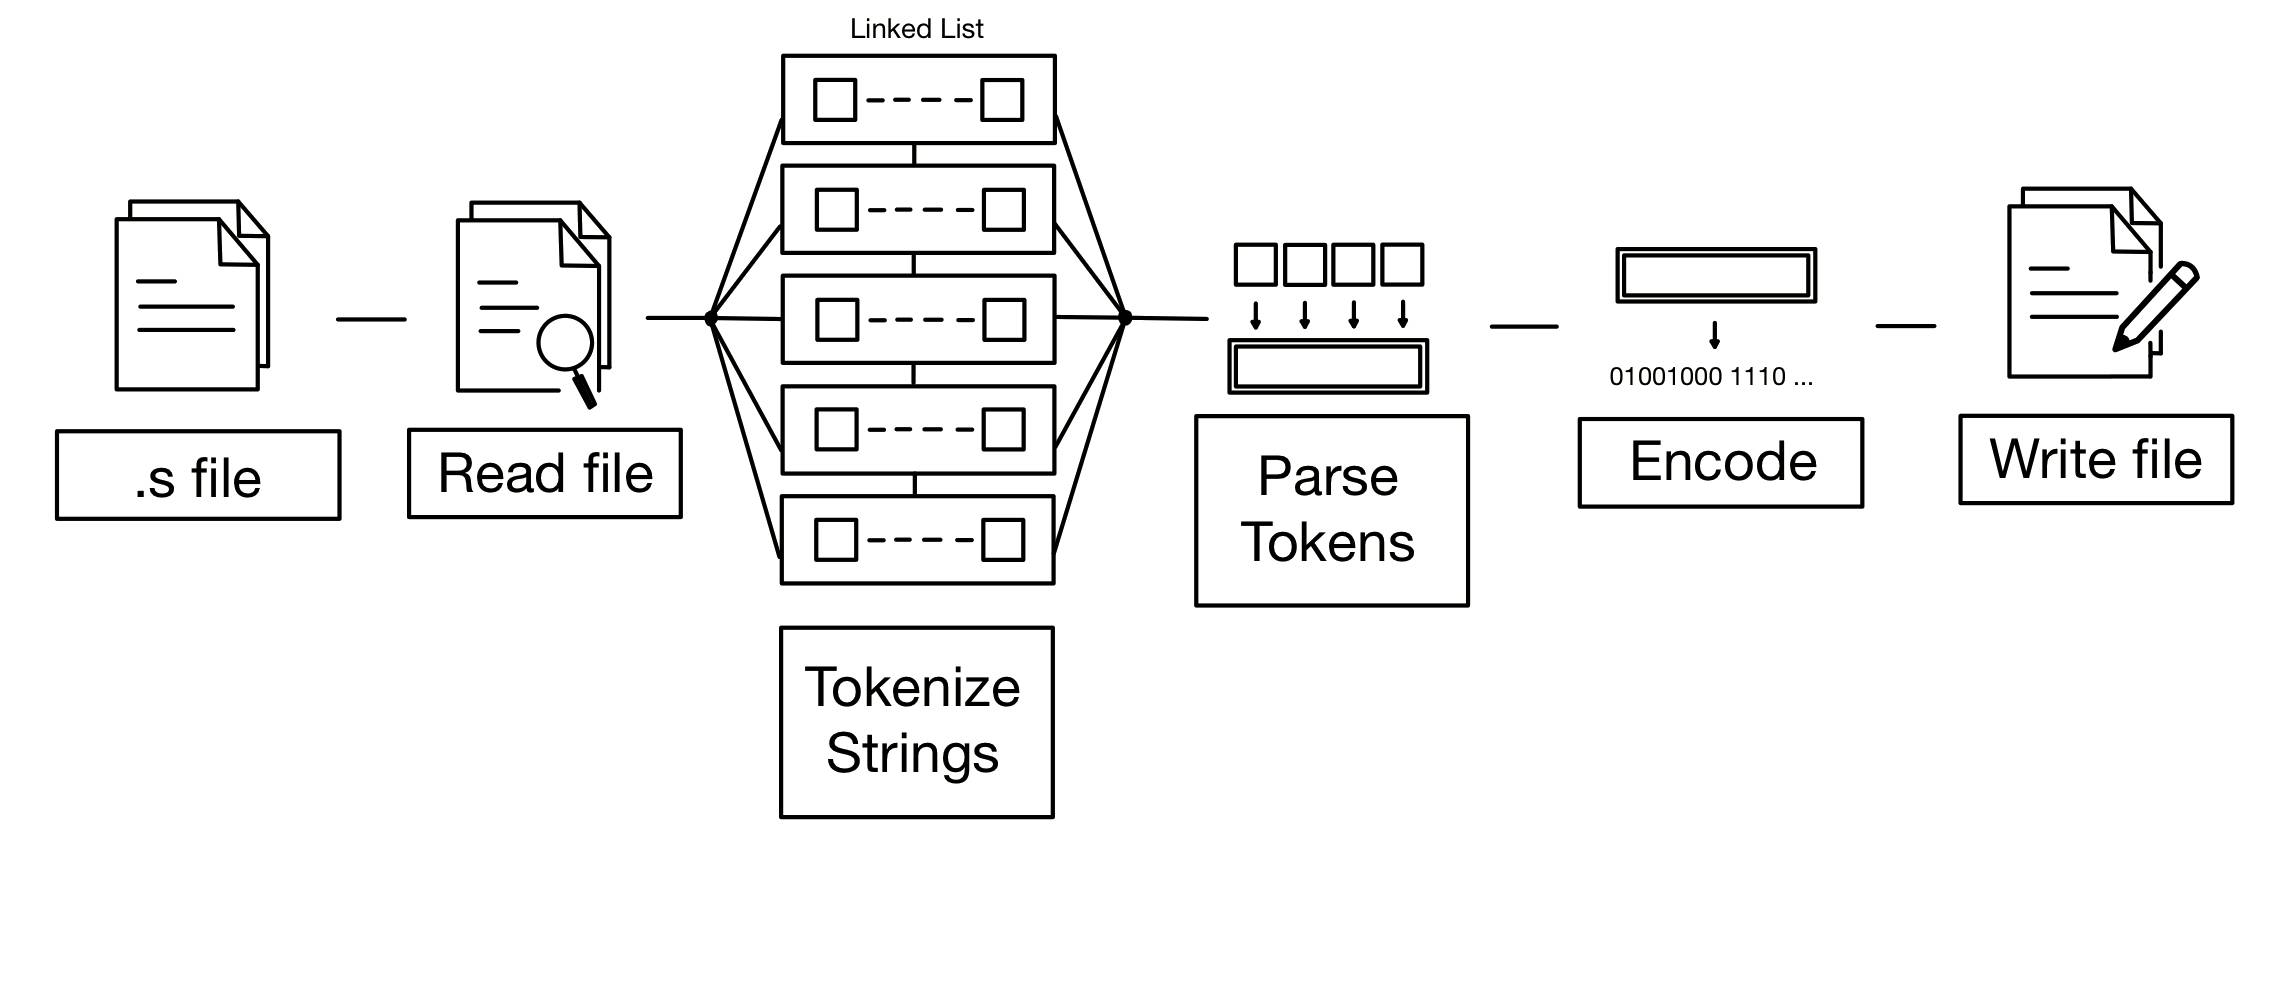
\includegraphics[width=15cm]{assembler_flow.jpg}
    \caption{Our 2-pass assembly process}
    \label{fig:assembler}
\end{figure}

\subsection{The implementation:}\label{Assembler implementation}
\subsubsection{Problems we overcame: }
A notable issue we faced was that we did not know how many lines there were in each source file, so we could not create an array of strings to store these instructions. To tackle this, we used a linked list to store the instructions instead. Since we took such an approach, we could then read through the source file once, converting each instruction in a tokenized form and inserting them into the linked list. Labels are inserted into our symbol table, and are not inserted into the linked list. This is the reason why we preferred a 2-pass approach over a 1-pass one.

\subsubsection{Improvements after weekly meetings: }
During our weekly mentor meetings, Professor Knottenbelt suggested that we move away from switch-case statements and delve into the world of functional pointers. We took the advice and incorporated suitable function pointers wherever possible. Figure \ref{fig:functional_pointers} shows how we have used functional pointers in our assembler, this example shows that the function attribute of the instruction function map points to the appropriate function which is \verb|parse_dataproc| in this case. The use of this method allowed for code modularity and also enabling object oriented programming features in our code base.

\begin{figure}[htp]
\centering
\begin{BVerbatim}
instr_func_map and = {
.code.dataproc_opcode = AND,
.function = &parse_dataproc /* FUNCTIONAL POINTER USED */
};
// continues for all operations below...
\end{BVerbatim}
\caption{Example of functional pointers in the assembler}
\label{fig:functional_pointers}
\end{figure}

\subsubsection{Tokenizer:}
Another interesting aspect of our assembler is how our tokenizer works. Before passing anything to \verb|tokenizer()|, we check that its not a label, it will always be an instruction line. Then we allocate contiguous memory to a \verb|token_list| which will store our tokenized instruction. Then, instead of using \verb|strtok_r()|, we used our own version - \verb|strbrk_r|. This choice was made due to two reasons:
\begin{enumerate}
    \item \verb|strtok_r()| isn't portable for pre-POSIX-2001 systems and it caused a lot of compilation issues on macOS.
    \item Our \verb|strbrk_r()| functions returns the delimiters inside the returned tokens, which was important to identify pre-indexed and post-indexed instructions. For example, \verb|strtok_r()| wouldn't return the square brackets in \verb|ldr r1, [r0]| when they are required for parsing purposes later on in the assembler process.
\end{enumerate}
A \verb|while| loop is used together with \verb|str_brk()|inside \verb|tokenizer()| to convert instruction strings into token lists. Any allocated memory is freed accordingly. When \verb|tokenizer()| is complete, the linked list will contain a token list in every node, each corresponding to an instruction in the source file in order.

\subsubsection{Parser and Encoder:}
We have decided to create multiple parser functions that handles different instructions. In order to access each function, we use a \verb|instr_func_map| datatype as mentioned in Figure \ref{fig:functional_pointers}. As mentioned earlier in sub-section \ref{The structure}, the symbol table is populated with these function mappings. This allows us to query the symbol table with an instruction name such as \verb|mov|, and have the symbol table return its corresponding \verb|instr_func_map| as shown in Figure \ref{fig:calling functions with func map}.


\begin{figure}[htp]
\centering
\begin{BVerbatim}
func_map = st_retrieve(labels, tokens->list[0].data.instr_name);
...
binary_instr = func_map->function(curr, func_map->code, labels);
\end{BVerbatim}
\caption{Retrieving func\_map data and calling the function through a function pointer}
\label{fig:calling functions with func map}
\end{figure}

All token lists produced by reading the source file will always begin with a token containing its instruction name. This is used to query the symbol table. This is why \verb|tokens->list[0]| is used to query the symbol table.

The parser works together with the encoder to produce a 32 bit binary value. This value will then be written to an output file.

% -------------------------------------
\section{Extension: Modelling a Distributed Ledger Cryptocurrency (ImpCoin) with a Concurrent Centralised Network}
\subsection{Description \& Real world usage:}

For our extension, we simulated a decentralised blockchain cryptocurrency called \textbf{ImpCoin}. The simulation relies on a centralised \verb|address node|, this acts like the server in a client-server model. It is responsible for distribution of all information on the ``decentralised'' blockchain. The reason why we decided on this implementation is mainly due to time constraints, we found out quite early on that implementing a fully decentralised network in C would require a lot more hours than we could spare. Along with essential blockchain and transaction functions, we also implemented basic concurrency in the network to allow mining and transactions to occur at the same time between multiple clients.

In the real world, all our transactions are monitored by a governing body and the majority of our money is regulated by regulatory bodies. This is not necessarily a good thing (that's a debate for another day !), this is where crypto fills the void in the market. Our system ensures a ``trustless'' system, this means that the uses on the network don't necessarily need to trust their peers; the consensus system ensures that the trust is built on the distributed ledger. Nobody is allowed to alter or delete anything form the shared ledger and any mining of blocks checks the transactions made on the network. The side-effect of having this shared currency is that transactions and transfers are lightning fast, easy and free of cost as \textbf{ImpCoin} has no middle man.

\subsection{The implementation:}
\subsubsection{High-level details:}

There are two main executables in our implementation. First, we have a \verb|node| which presents the user with an interactive prompt, allowing them to mine $n$ blocks, make transactions and print out internal state for debugging purposes. Each \verb|node| stores a copy of their own blockchain, which contains a linke

In order to create a blockchain network in C, we needed to implement several things:
\begin{itemize}
    \item Suitable data structures to model blocks, transactions, a variable length list of transactions and a blockchain. We were able to make use of some of our experiences and code in the assembler for this, especially in implementing linked data structures.
    \item Functions to serialise 
\end{itemize}

\begin{figure}[htp]
    \centering
    \subfigure[Centralised]{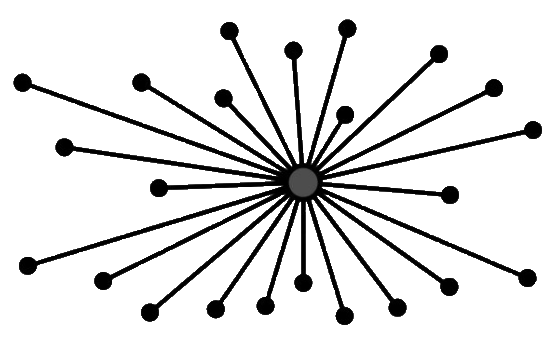
\includegraphics[width=30mm]{centralised.png}}
    \qquad
    \subfigure[Decentralised]{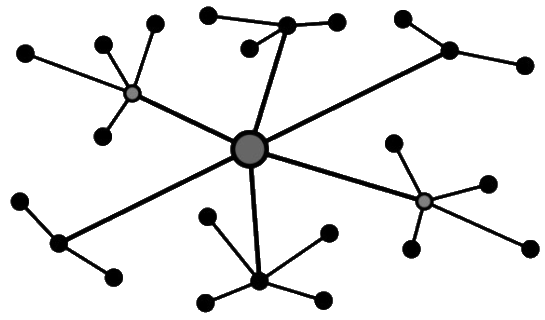
\includegraphics[width=30mm]{decentralised.png}}
    \caption{Network types}
    \label{fig:network-types}
\end{figure}

\subsubsection{Issues we overcame: }
\lipsum[1-1]

\subsection{Testing and Effectiveness:}
After setting up the basic skeleton of the extension, we also got started on our test suite. The constantly evolving test suite contains basic building blocks which are then used for more complex tests. For example, \verb|test_string()| (checks string equality) is used in \verb|test_hash()| (checks hash equality) which is utilised in \verb|test_hash_equality()| which checks whether the hashes of the passed in blocks are equal. We have tried to use this "ground up" approach wherever possible as it reduces code duplication. Figure \ref{fig:test-example} shows part of the command line output of the \verb|testrunner| when its run (the \texttt{\textcolor{BOLDRED}{FAIL}} is just an example, all our cases pass!). We use escape sequences to output colourful text in the terminal.

Our test suite helped us catch a lot of obscure bugs which we hadn't thought of before, and it was also our first taste at Test Driven Development. A lot of really enjoyed the process of writing tests before typing code because it gave us a better idea on how to get started. Apart from the test suite, we also stress tested our system with multiple terminals mining at once to see if everything functions smoothly and relatively quickly. It was also satisfying to hit smaller goals more often as it boosted our enthusiasm throughout the journey.

\begin{figure}[htp]
\centering
\begin{BVerbatim}[commandchars=\\\{\}, fontsize = \small]
-----\textcolor{BOLDBLUE}{SERIALIZE/DESERIALIZE TESTS}-------------------------------------
TEST - Transactions are equal on both ends : \textcolor{BOLDGREEN}{OK}
TEST - Linked list of transactions is equal on both ends : \textcolor{BOLDGREEN}{OK}
TEST - Genesis block is equal on both ends, with hash : \textcolor{BOLDGREEN}{OK}
TEST - Blockchain is equal on both ends : \textcolor{BOLDRED}{FAIL}
---------------------------------------------------------------------
\textcolor{BOLDYELLOW}{PASSING: (3/4) tests}
---------------------------------------------------------------------
\end{BVerbatim}
\caption{Example of our Test Suite}
\label{fig:test-example}
\end{figure}

\newpage
% -------------------------------------
\section{Group Reflection}
\subsection{Effectiveness of communication and division of work:}

As discussed in the Emulator Interim Checkpoint, we have been using our Discord server for all our communications (text, audio and video). Our setup was more than successful in our opinions, it was the perfect balance of professional and casual as we were mindful of dividing our time between work and leisure. Whether it be late night talks about the countries we come from or sending memes in our \verb|#random| channel. During our almost 24/7 text correspondence, we spend approximately 6 to 8 hours on call to program, relax, make design decisions or brainstorm extension ideas. We are also very careful that we don't strain ourselves so we make sure that we collectively take breaks, which has in fact increased our productivity generally. In the assembler implementation phase of our project, we considered using a more thought out process of collaboration; we came across the concept of pair programming. This technique has a \textit{driver} (one who writes the code) and an \textit{observer} (one who reviews each line of code typed by the driver). It really helped us understand the code better, which in turn meant we could optimise/ refactor it easily. It also reduced the number of errors per line.

In the assembler, we decided to split up larger parts of the project. Kavya was in charge of creating the linked list which is essentially the backbone of the assembler, Yelun was in charge of the symbol table and Ashvin and Siddhant were in charge of the tokenizer. This way, we could essentially branch out from \verb|master| and then merge all branches together and fill any cracks we neglected. This method saved us a lot of time as everyone was independently coding at their own pace (which also allowed everyone to make suitable unit test cases in \verb|testrunner.c|). Another effective technique we used was making meaningful commit messages and merge request descriptions which come handy when we want to clarify a merge conflict or any gaps in understanding. Overall, we are all very happy with how well we have done in the project and the amount of progress we have made both as a team and personally.

\subsection{Future improvements:}
Although our group was efficient, there were some aspects that we could have incorporated for a better result. For example, we could have utilized pair programming a little more during debugging sessions and larger aspects of the project that required design choices and second opinions. This would have sped up the process and also ensured a more optimal outcome.

Additionally, we could have managed our time more efficiently in order to get the project done well before the deadline. This would have left us enough time to incorporate some final refactoring and other minute details that were required for completion of the project. This management would have been possible if we had paced out our work during the initial part of the project, to avoid burn-out and a slower pace for the rest of the project. 

Furthermore, the group could have spent a little more time researching about the best way to solve a problem or to pick between design choices, in order to avoid working out one implementation before changing it to another one. The research could have helped save more time. 

Overall the project was fairly well-coordinated and we had numerous achievements and learning experiences along the way, which every member can take forward into future projects and into the work environment as well.

% -------------------------------------
\section{Individual Reflections}
\subsection{Ashvin:}
\lipsum[1-1]
\subsection{Kavya:}
The group project was rather well coordinated and organized compared to the ones I've done before. Every member of the group has come a long way since the beginning of the project, with new perspectives and skills that we would not have thought we would acquire. Every member had their own opinions that were portrayed in such a way that they came together to find the most optimal solutions to a problem instead drowning other opinions out. The work was efficiently split and the pace was flexible depending on every team member's requirements. Despite the time zone differences and lack of in-person communication, the communication was handled professionally yet informally, allowing us to work in an environment of comfort and mutual respect.

I certainly learnt the importance of division of work and concurrent individual working, and when it should be used as opposed to pair programming. Every member was very self-motivated and eager to help which was a major factor that contributed to our efficiency. The willingness to listen, consider, suggest and help is something I would like to take forward from this group project and my teammates.  We recognized our strengths and weaknesses and used them to compliment each other and build the project. I was personally stronger with building data structures and Overall I am proud of how far we have come and the achievements and learning experiences we've had along the way. We learnt not only from the project but also from each other. The importance of communication, passion and respect truly came to light through the project and I will certainly incorporate these experiences in future projects.

\subsection{Siddhant:}
Overall, I am very satisfied with our project as it is the product of self motivated and guided work. Recalling back to the first 2 days of the project, some of us didn't know how to handle git branches and merge requests; so to see how far we have come since then is very rewarding. Not only did we finish the ARM emulator and assembler in time but we also incorporated the optional test cases. Our chemistry as a group worked very well because we set aside enough time in the day to bond as friends and not just teammates. This allowed free flowing conversations during brainstorming meetings and also enabled everyone to speak their mind freely without feeling anxious especially in a time like this where none of us have ever met each other in person.

As some members of our team had previous experience in industrial programming, they imparted that knowledge with the rest of us which encouraged good coding and git practices (like properly formatted git commit messages which convey suitable amounts of information within 1 sentence). I will definitely be carrying forward these valuable soft skills in future projects and hopefully in the workplace. If I were to do this project again, I would probably further divide the work for Assembler as pair programming held us back in terms of time, on the other hand, pair programming reduced the number of bugs we had during testing as there were 2 pairs of eyeballs on 1 piece of code.

\subsection{Ye Lun:}
I have participated in group projects for development in the past with supervisors who observed my work consistently and guided me to the point of hand holding. This C group project was different, where most of our guidance from our mentor centered around improving what we already had accomplished. The initial project structure, and many other aspects were decided by ourselves after multiple discussions. Making these decisions was a difficult yet fulfilling experience since we were unaware of what is optimal, which enabled us to generate a large number of ideas and methods to approach the problem.

Our group coordination started great, and kept improving over time. Initially, We discussed the work that we planned to do and each member would proceed to work on their own segment, before presenting their code to everyone else. These code reviews were useful as it helped us understand why the code is written a specific way, and more people can catch any undetected bugs. This then gave us the idea to do some pair and group programming sessions for when we worked on the assembler. We therefore initiated pair and group programming sessions when working on the assembler so we could understand what one another is doing in real time. These were more spontaneous and it helped to further improve our group cohesiveness. This practice carried over into building our extension as well. These sessions do come at a cost of time, but I feel that the benefit of being on the same page as a small group outweighs the time loss, and I hope to bring this practice into future projects.

\end{document}